%!TeX program = xelatex
\documentclass[12pt,hyperref,a4paper,UTF8]{ctexart}

\usepackage{UCASReport}
\usepackage{enumitem}
\usepackage{booktabs}

\setlist[1]{
    itemsep = 0pt,
    partopsep = 0pt,
    parsep = 0pt,
    topsep = 5pt,
    leftmargin = 2em,
    labelsep = 0.25em
}

\newcommand{\barline}[1]{\overline{#1\rule{0pt}{1.5ex}}}

%%-------------------------------正文开始---------------------------%%
\begin{document}

%%-----------------------封面--------------------%%
\cover

%%------------------摘要-------------%%
%\begin{abstract}
%
%在此填写摘要内容
%
%\end{abstract}

\thispagestyle{empty} % 首页不显示页码

%%--------------------------目录页------------------------%%
\newpage
\tableofcontents

%%------------------------正文页从这里开始-------------------%
\newpage

%%可选择这里也放一个标题
%\begin{center}
%    \title{ \Huge \textbf{{标题}}}
%\end{center}


\section{分工介绍}
\subsection{中期工作}

\begin{itemize}
    \item 赵XX：整理材料
    \item 李XX：调查文献研究
    \item 蔡XX：汇报
    \item Illusionna：制作幻灯片
\end{itemize}



\subsection{答辩工作}
\begin{itemize}
    \item 赵XX、李XX：VR 采集眼动数据、多维度分析、机器学习
    \item 蔡XX：深度学习
    \item Illusionna：撰写内容制作幻灯片并答辩
\end{itemize}



\subsection{报告工作}
各自完成自己相关部分的论文内容，Illusionna 汇总所有材料、\LaTeXe 排版文章。



\section{课题背景及意义}
\subsection{研究背景}
随着全球人口老龄化趋势的日益加剧，阿尔兹海默症（Alzheimer's Disease, AD）及轻度认知障碍（Mild Cognitive Impairment, MCI）的患病率正以前所未有的速度上升，给社会医疗体系和家庭带来了沉重的经济与心理负担。然而，现有的临床诊断手段在早期发现方面存在显著局限性。一方面，诊断高度依赖 MMSE（简易精神状态检查）和 MoCA（蒙特利尔认知评估）等传统主观量表，此类测试不仅人工耗时长，且极易受到受试者文化程度、心理状态及主观干扰的影响。这些量表虽然普及，但在捕捉极早期认知衰退的灵敏度上存在争议\cite{folstein1975mini}。另一方面，当认知功能受损能够被此类量表捕捉时，患者通常已进入病程中晚期，错失了早期干预的最佳时机。因此，探索一种客观、可量化、非侵入式且具备高灵敏度的早期风险预警方法，已成为神经科学与智能人机交互领域的急迫需求。

\subsection{研究意义}
平滑追随运动（Smooth Pursuit）是指视觉系统对运动目标进行连续追踪的能力，其生理基础涉及大脑额叶（FEF）、顶叶（PPC）及小脑的高效协同。研究指出，动眼神经系统的完整性是评价中枢神经系统功能的重要窗口\cite{leigh2015neurology}。

\begin{itemize}
    \item \textbf{临床敏感性}：研究表明，认知功能的退化（如 AD/MCI）会直接导致动眼神经系统的注视增益降低、神经反应延迟增加。相比传统量表，眼动特征能捕捉微秒级的早期神经功能病变，具有极高的灵敏度。
    \item \textbf{虚拟现实（VR）的生态效度}：本研究利用沉浸式 VR 环境模拟真实的乒乓球和网球场景，相比实验室中简化的“圆点运动”，此类任务能有效激发受试者的自然认知负荷，提升测试的生态效度。虚拟现实技术被证明能比传统实验室任务更有效地诱发与日常生活相关的认知负荷\cite{parsons2015virtual}。
    \item \textbf{交互特征的高频标准化}：利用内置眼动仪捕捉 50Hz 的高频数据，可以在排除物理环境干扰的同时，提取视线与目标在三维空间中的时空耦合特征，解决了传统测试受主观干扰大的痛点。
\end{itemize}

\subsection{核心动机与任务目标}
传统眼动分析多聚焦于以屏幕坐标为参照的静态热力图，分析“人看了哪里”，却忽略了目标本身的运动特征。本研究的核心动机在于实现从“视觉注视”向“动态追踪”的行为范式转换，关注视线与目标间的相对位移，从而提取轨迹一致性、滞后性、曲折度等具备病理可解释性的动态特征。

本研究的具体任务包括：

\begin{enumerate}
    \item \textbf{构建映射范式}：建立以运动轨迹为基准的行为分析范式，实现屏幕坐标向目标中心坐标的统一。
    \item \textbf{多维特征量化}：比较健康对照组（HC）、MCI 组与 AD 组在追踪特征上的差异，涵盖生理负荷、运动学控制及频域稳定性。
    \item \textbf{模型自动化评测}：基于机器学习构建自动化分类评测模型，验证动态眼动行为作为早期筛查生物标记物的有效性。
\end{enumerate}


















\section{VR 采集眼动数据}
本研究基于 Unity 3D 引擎构建了一套沉浸式虚拟现实（VR）实验采集系统，并选用 PICO 3 VR 一体机作为核心交互终端。

在采集程序的开发环节，我们利用 PICO Unity Integration SDK 搭建了 XR Interaction 交互框架。通过编写 C\# 脚本，系统能够以高频率实时获取用户的头戴显示器（HMD）及手柄控制器的 6 自由度（6DoF）空间位姿数据（包括三维坐标 Position 和四元数旋转 Rotation）。同时，为了保证实验流程的标准化，我们在 Unity 中设计了严格的场景状态机，用于控制刺激源的呈现时间、交互逻辑及用户反馈的 UI 界面，确保每一位受试者在完全一致的虚拟环境中进行操作。

在 VR 端与上位机的通讯环节，为了实现数据的实时监控与持久化存储，我们设计了一套基于 TCP/IP 协议的局域网通讯架构。PICO 3 设备作为客户端，通过 Wi-Fi 6 网络与作为服务端的 PC 上位机建立 Socket 连接。采集程序将传感器原始数据实时序列化为 JSON 格式数据包，并通过多线程异步传输机制发送至上位机；上位机端则开发了相应的数据接收与解析模块，负责实时校验数据完整性并将其写入本地数据库，从而实现了从 VR 终端到 PC 端的高效、低延迟数据链路。

在系统测试与初步采集阶段，我们招募了数名年龄分布在 22 至 23 岁的青年受试者进行了预实验。尽管采集程序运行稳定且通讯链路畅通，但鉴于实地采集样本数量较少，难以满足深度学习模型训练对数据多样性与泛化能力的严苛要求，同时也为了规避小样本带来的统计偏差，本研究最终决定采用导师提供的标准数据集进行后续的模型训练与分析工作。

该数据集来源于医院临床采集，包含约 70 余名受试者的高质量多模态数据，具有极高的医学研究价值。根据数据集的统计信息，该数据源具有以下显著特征：
受试者分布广泛且均衡：数据集涵盖了 HC（健康对照组）、MCI（轻度认知障碍组）、mildAD（轻度阿尔茨海默病组）、moderateAD（中度阿尔茨海默病组）以及 MMD（轻中度痴呆组）等多个认知层级。这种多分类的梯度设置，使得模型能够学习到从健康到疾病演变过程中的细微行为差异。

人口学特征符合发病规律：受试者年龄主要分布在 55 岁至 82 岁之间涵盖了从小学到大学的不同受教育程度，符合 AD 疾病的高发人群画像，具有极高的生态效度。



\section{轨迹可视化与多维度分析}
\subsection{轨迹可视化}
\subsubsection{数据清洗与平滑}
原始眼动数据与球体追踪数据可能存在丢帧或噪声。首先，我们采用线性插值填补缺失的数据点。随后，为了消除高频抖动并保留运动趋势，对 $(x, y)$ 坐标应用了窗口大小为 3 帧的移动平均滤波器，见\autoref{eq-average-filter}：
\begin{equation}
    \barline{P}_{\text{smooth}}(t)=\dfrac{1}{w}\sum_{i=-k}^{k}P(t+i) \label{eq-average-filter}
\end{equation}

其中 $P(t)$ 为当前时刻坐标，$w$ 为窗口大小。



\subsubsection{坐标系映射与变换}
由于眼动仪采集的数据基于屏幕中心为原点的坐标系（$1280\times720$），而目标视频为左上角为原点的像素坐标系（$1920\times1080$），因此需要进行空间变换。变换公式如下\autoref{eq-transform}：
\begin{equation}
    \begin{cases}
        x'=\left(x_{\text{raw}}+\dfrac{W_{\text{src}}}{2}\right)\cdot S_{x}
        \\[10pt]
        y'=\left(\dfrac{H_{\text{src}}}{2}\pm y_{\text{raw}}\right)\cdot S_{y}
    \end{cases} \label{eq-transform}
\end{equation}

其中，$(x_{\text{raw}}, y_{\text{raw}})$ 为原始眼动坐标，$(W_{\text{src}}, H_{\text{src}})$ 为采集设备分辨率；$(S_{x}, S_{y})$ 分别为水平和垂直方向的缩放因子（本研究中 $S_{x}=S_{y}=1.5$）。考虑到坐标系定义的差异，公式中对 Y 轴进行了翻转修正，以确保注视点垂直方向运动与视频画面一致。



\subsubsection{时空对齐与渲染}
由于眼动仪采样率与视频帧率（FPS）不一致，我们通过时间戳归一化将眼动数据映射到对应的视频帧索引，在可视化输出中：

\begin{itemize}
    \item 注视点：使用蓝色半透明圆形标记，以避免遮挡关键比赛细节。
    \item 网球：使用橙色实心圆形标记。
    \item 运动轨迹：为了展示运动的速度感与路径历史，系统绘制了长度为 20 帧的“彗星尾迹”，尾迹宽度随时间衰减，从而清晰呈现运动方向，如\autoref{fig-left} 和\autoref{fig-right} 人眼跟踪球轨迹示意图。
\end{itemize}

\begin{figure}[htbp]
    \centering
    \begin{minipage}{0.48\textwidth}
        \centering
        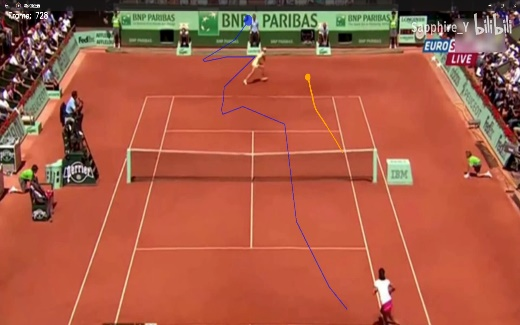
\includegraphics[width=\linewidth]{./figures/left.png}
        \caption{人眼跟踪球轨迹示意图（左）}\label{fig-left}
    \end{minipage}
    \hfill
    \begin{minipage}{0.48\textwidth}
        \centering
        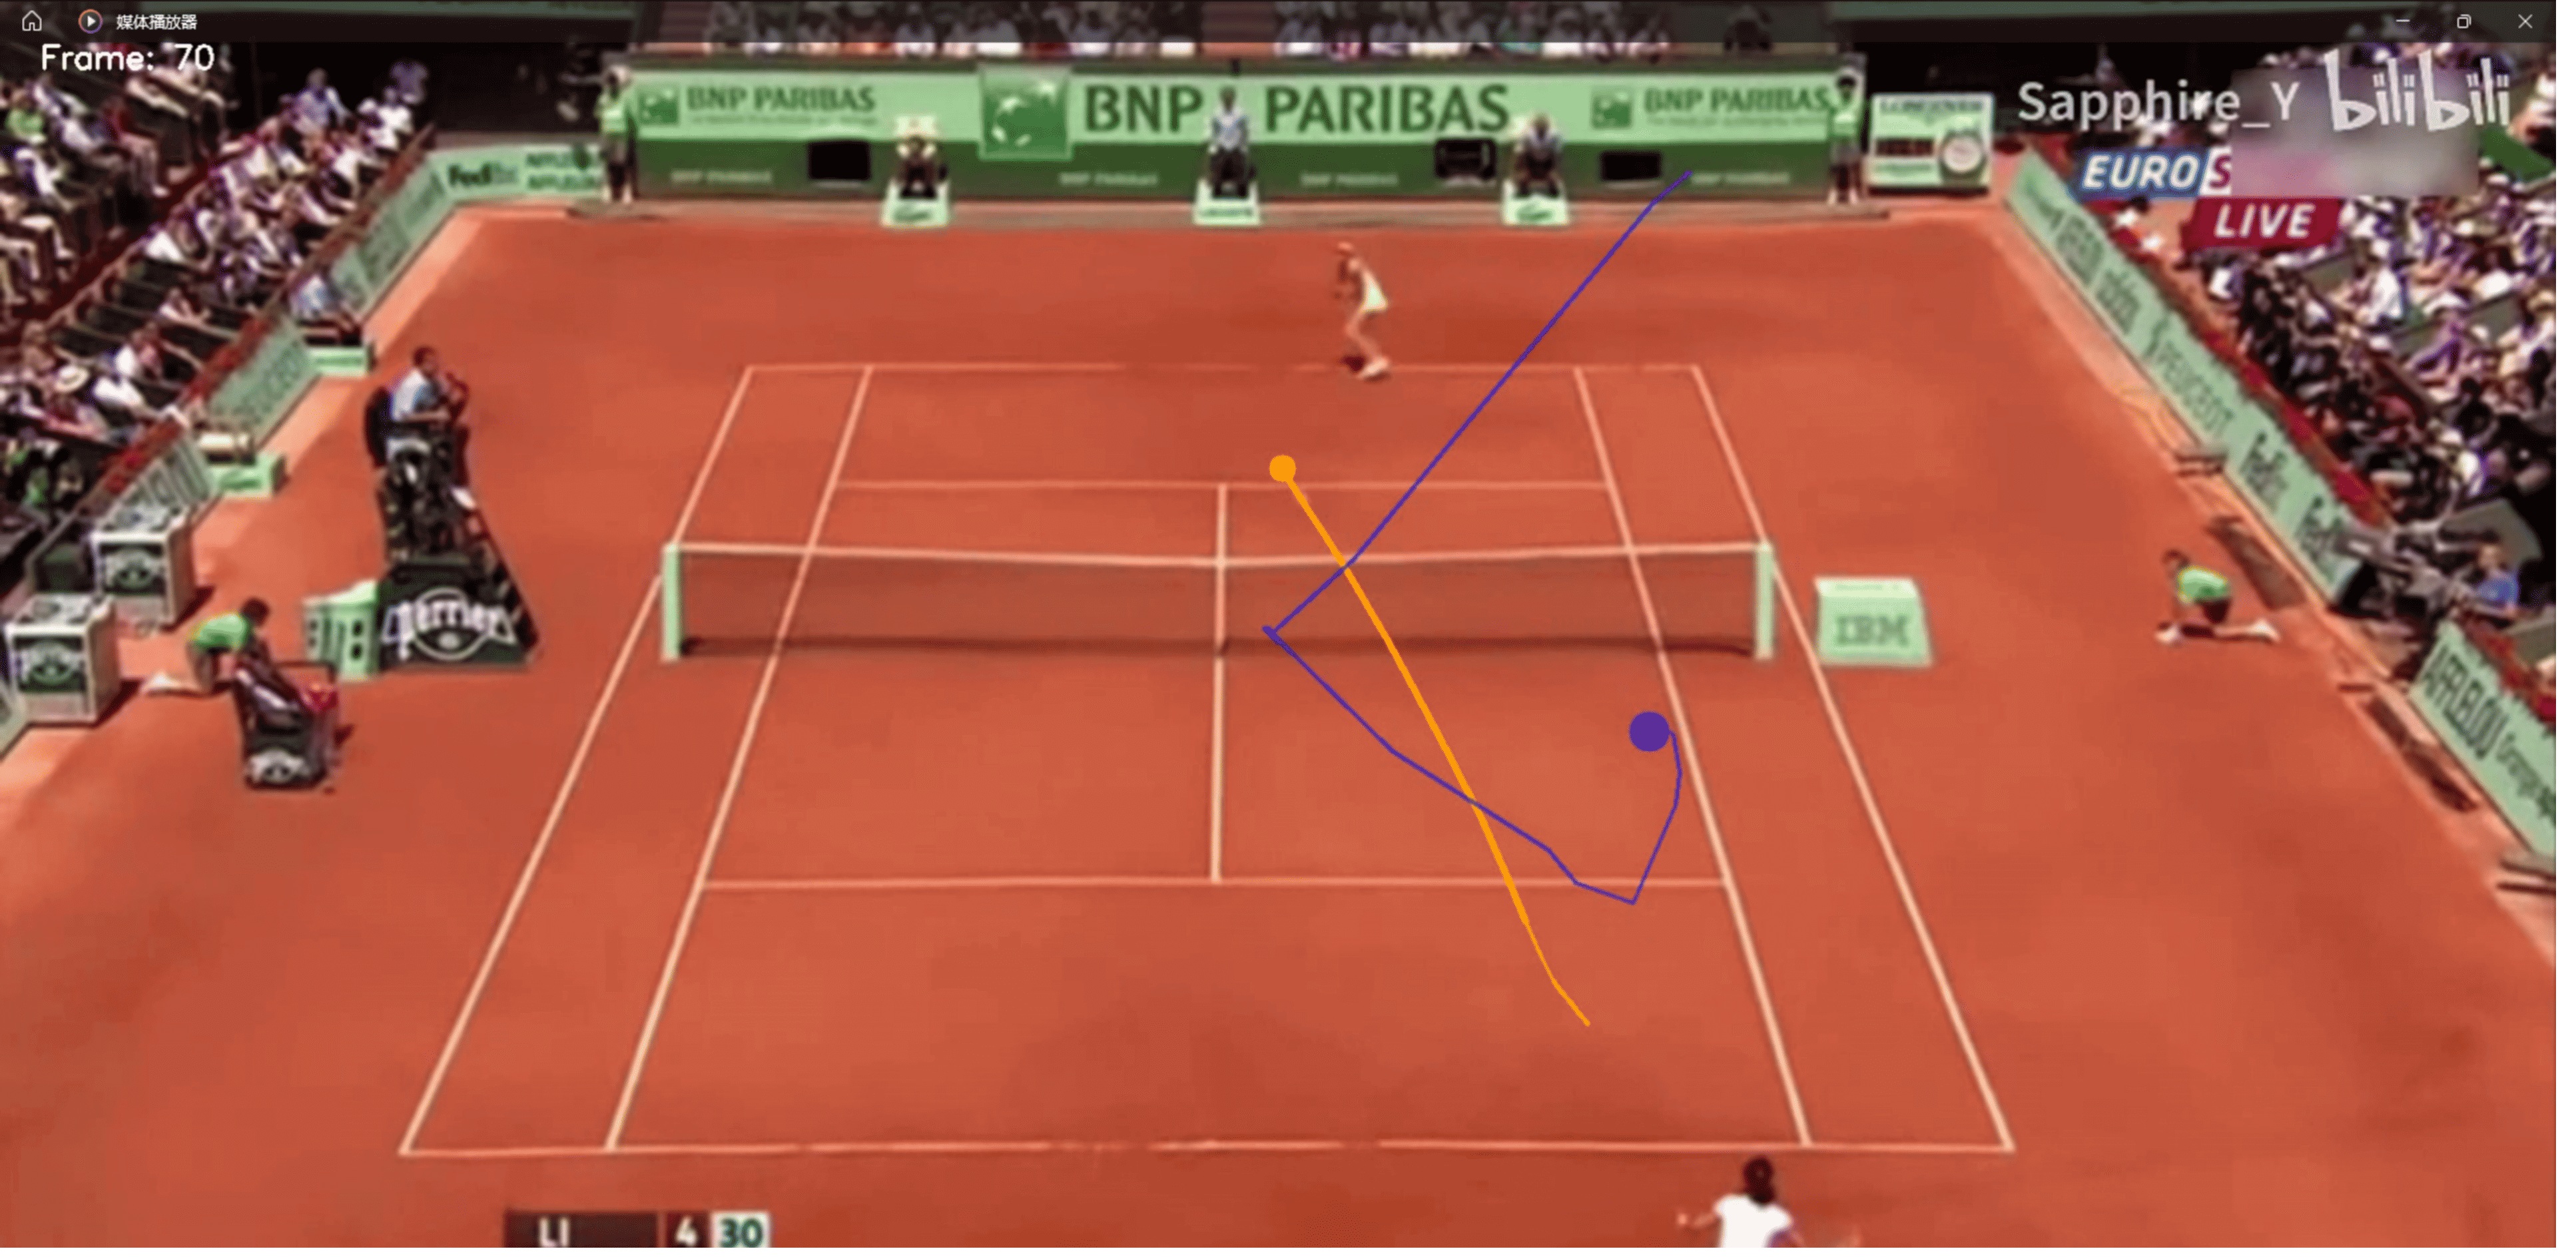
\includegraphics[width=\linewidth]{./figures/right.png}
        \caption{人眼跟踪球轨迹示意图（右）}\label{fig-right}
    \end{minipage}
\end{figure}



\subsection{多维度分析}
\subsubsection{视觉误差分析}
为确保多源数据的时空一致性并量化视觉追踪表现，本研究实施了标准化的数据处理流程。首先，针对眼动仪（50 Hz）与视频刺激材料（30 Hz）采样率的差异，采用线性插值算法将视频中球体的物理轨迹坐标映射至眼动数据的时间轴，实现了注视点与目标位置的帧级同步。在此基础上，定义“注视点-目标距离误差”作为核心指标，通过计算每一有效时间点 $t$ 的注视坐标 $(x_{g}, y_{g})$ 与球体坐标 $(x_{b}, y_{b})$ 之间的欧几里得距离，定义如\autoref{eq-euclidean-distance} 所示：
\begin{equation}
    \text{Error}_{t}=\sqrt{\displaystyle(x_{g}-x_{b})^2+(y_{g}-y_{b})^2} \label{eq-euclidean-distance}
\end{equation}

来量化追踪精度，为排除设备校准失效或受试者配合度低导致的系统性偏差，研究采用了基于分组统计分布的异常值清洗策略，剔除超出组内均值特定标准差范围（$\mu\pm N\sigma$）的极端样本。最后，数据分析采用双层级聚合方法，优先计算每位参与者的加权平均误差，随后依据临床诊断标签（如 HC、MCI、AD 等）汇总计算各组别的总体均值、标准差及样本量，以评估不同认知状态下的视觉运动控制水平如\autoref{tab-error} 所示。

\begin{table}[htbp]
    \centering
    \setlength{\tabcolsep}{16pt}
    \renewcommand{\arraystretch}{1.2}
    \caption{视觉误差分析表}\label{tab-error}
    \begin{tabular}{cccc}
        \bottomrule[1.5pt]
        组别（Group） & 样本量（$N$） & 平均误差 & 标准差 \\
        \midrule[0.75pt]
        HC（健康对照组） & 31 & 248.95 & 27.52 \\
        MCI（轻度认知障碍） & 21 & 239.36 & 33.72 \\
        MMD（轻度情绪障碍/抑郁） & 10 & 234.09 & 30.46 \\
        mildAD（轻度阿尔茨海默病） & 9 & 250.96 & 35.66 \\
        moderateAD（中度阿尔茨海默病） & 2 & 225.64 & 10.26 \\
        \toprule[1.5pt]
    \end{tabular}
\end{table}

尽管本研究量化了视线追踪的平均欧几里得误差，但组间统计结果显示，单一的“平均误差（Mean Error）”指标在区分健康对照组（HC）与认知障碍组（MCI/AD）方面表现出显著的局限性。具体而言，各组的平均误差数值高度重叠（例如 HC 组为 248.95px，而 mildAD 组为 250.96px），差异缺乏显著的统计学区分度，这可能是以下原因：

指标的粗粒度掩盖了细节：平均值作为一种聚合统计量，平滑了追踪过程中的瞬时波动。患者可能在大部分时间内能够完成简单的视觉跟随，但在快速变向或高速运动时刻的“微观”眼动异常被整体平均值所稀释。

视觉任务的代偿效应：简单的球体追踪属于反射性较强的“由下而上”视觉任务，早期认知障碍患者可能调动了额外的注意力资源进行代偿，从而在宏观空间准确度上维持了与健康人相似的水平。



\subsubsection{非线性误差与拓扑分析}
鉴于常规的欧几里得平均误差在平滑了瞬时波动后难以有效区分早期认知障碍亚型，本研究构建了一个融合动态响应、非线性复杂度与空间拓扑的多维特征分析框架。该框架旨在从不同维度捕捉神经退行性疾病在动眼控制回路中的细微受损特征。

为了评估平滑追踪眼动系统的闭环控制效率，本研究引入速度增益指标。该指标量化了眼动速度对目标速度的跟随能力。设 $V_{\text{gaze}}(t)$ 和 $V_{\text{target}}(t)$ 分别为 $t$ 时刻注视点与目标的瞬时速度模长，则速度增益定义如\autoref{eq-gain}：
\begin{equation}
    \text{Gain}=\dfrac{\displaystyle\dfrac{1}{T}\sum\limits_{t=1}^{T}V_{\text{gaze}}(t)}{\displaystyle\dfrac{1}{T}\sum\limits_{t=1}^{T}V_{\text{target}}(t)} \label{eq-gain}
\end{equation}

为揭示动眼神经控制系统的稳定性与随机性，研究采用非线性动力学指标样本熵对误差时间序列 $X=\{x_1,\ x_2,\ \ldots,\ x_{N}\}$ 进行分析，样本熵衡量了序列产生新模式的概率，样本熵已广泛应用于生物医学信号的复杂性分析，能有效区分病理状态下的生理波动\cite{richman2000physiological}，其计算公式如下\autoref{eq-sample}：
\begin{equation}
    \text{SampEn}(m,r,N)=-\ln\left[\dfrac{A^{m}(r)}{B^{m}(r)}\right] \label{eq-sample}
\end{equation}

其中，$m$ 为嵌入维数（取值 2），$r$ 为相似度阈值（取 $0.2\times SD$），$B^{m}(r)$ 为序列中匹配长度为 $m$ 的模板数量 $A^{m}(r)$ 为匹配长度为 $m+1$ 的模板数量。

区别于均值误差对整体表现的平均化，豪斯多夫距离用于捕捉注视轨迹集合 $G$ 与目标轨迹集合 $B$ 之间的最大空间失配，即“最差情况”，该度量方法在轨迹相似度评价和计算机视觉目标识别中具有较强的稳健性\cite{huttenlocher2002comparing}。其定义为双向距离的最大值，如下\autoref{eq-hausdorff} 所示：
\begin{equation}
    H(G,B)=\max\left[\sup_{g\in G}\inf_{b\in B}d(g,b),\ \sup_{b\in B}\inf_{g\in G}d(b,g)\right] \label{eq-hausdorff}
\end{equation}

如\autoref{fig-hausdorff} 非线性误差分析图所示，综合分析各类动眼指标发现，轻度阿尔茨海默病（mildAD）组表现出独特的神经动力学受损模式。速度增益显著的高离散度揭示了患者动眼系统在“追踪滞后”与“代偿性扫视”间频繁切换的不稳定性，反映了顶叶-额叶注意网络对速度信号整合能力的衰退。患病组显著升高的样本熵表明其神经控制信号中混入了更多随机噪声，暗示了持续注意力维持过程中的系统无序性增加。最后，豪斯多夫距离中的极端异常值捕捉到了间歇性的大幅度视线丢失事件，这可能与海马体及内嗅皮层受损导致的空间工作记忆缺陷密切相关。上述结果共同证实，动眼控制的非线性与拓扑异常是反映早期神经退行性病变的敏感生物标记。

\begin{figure}[!htbp]
    \centering
    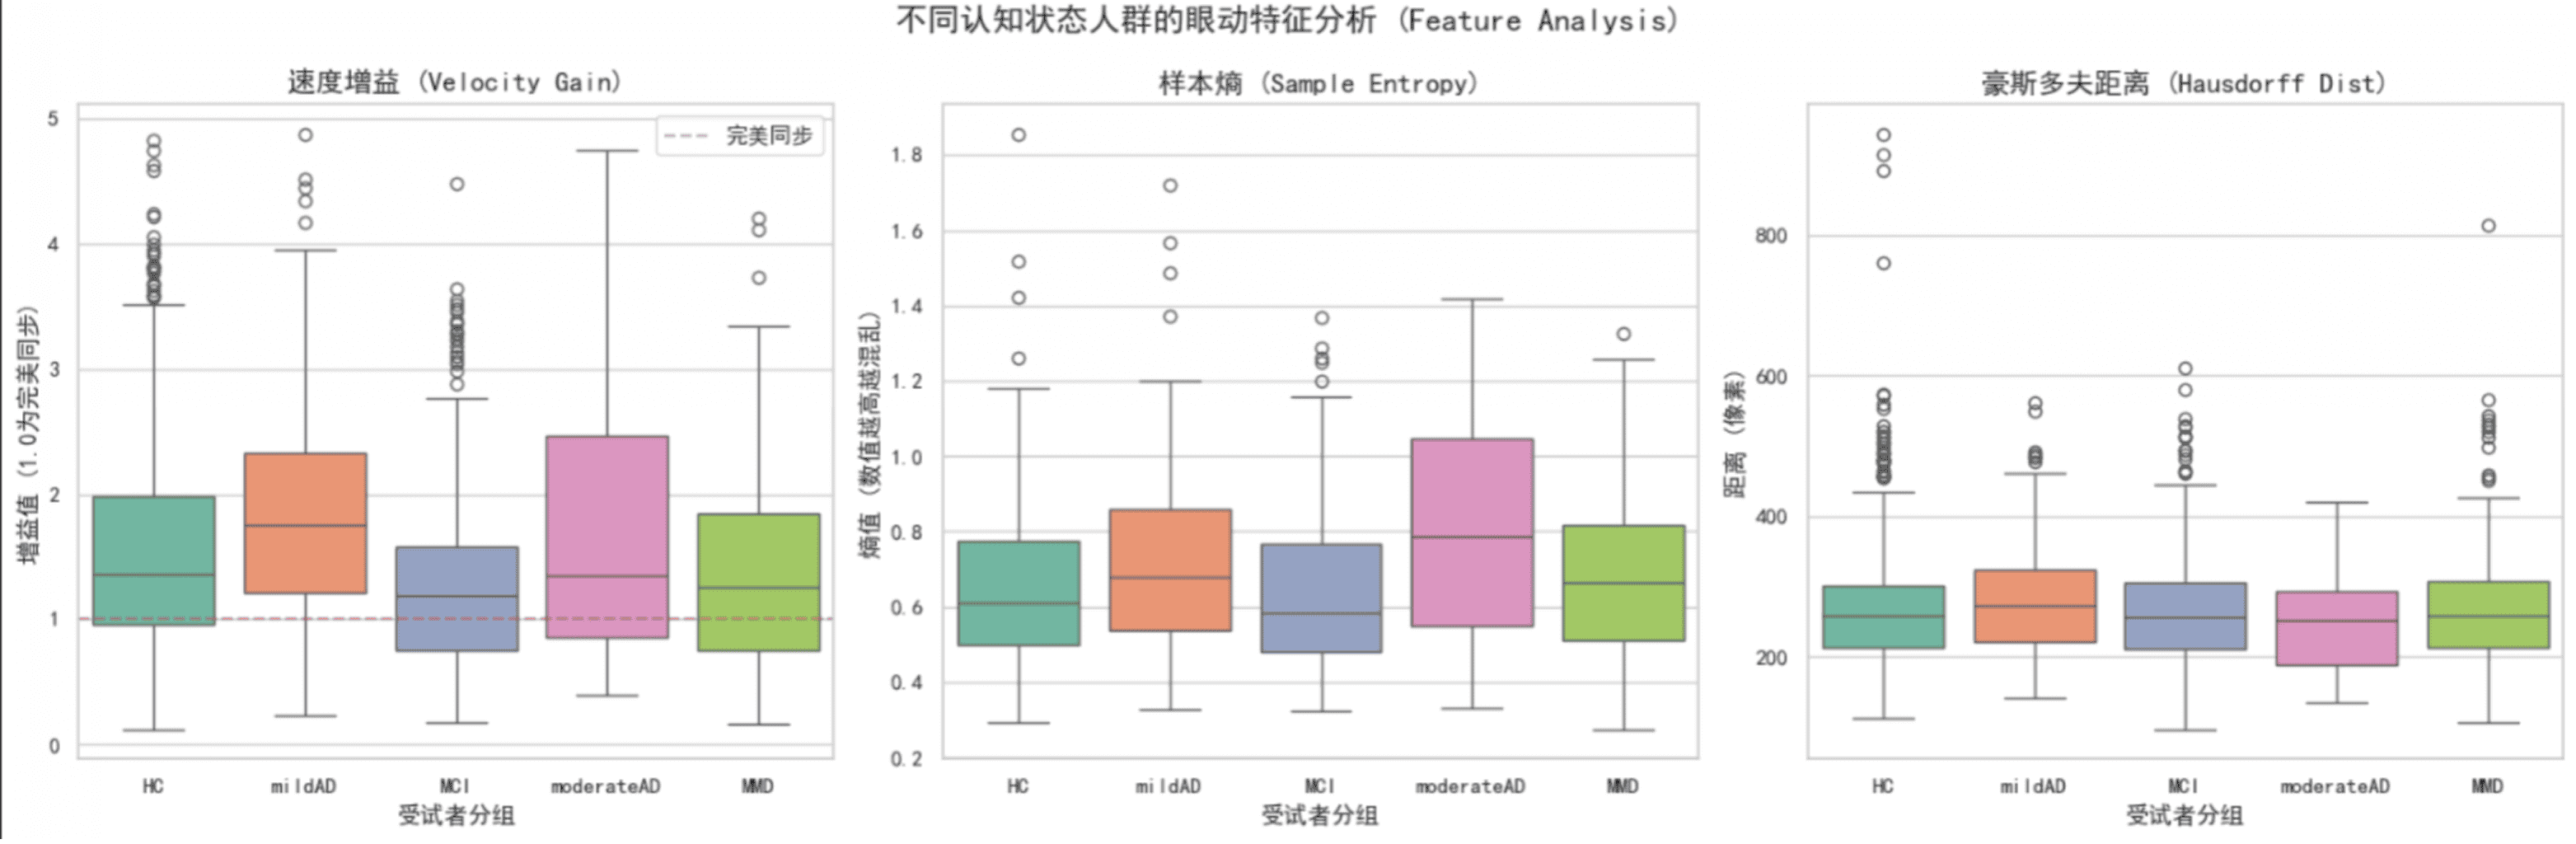
\includegraphics[width=0.95\textwidth]{./figures/hausdorff.png}
    \caption{非线性误差分析图}\label{fig-hausdorff}
\end{figure}



\subsubsection{注视分布特征区别分析}
不同认知状态人群的注视分布特征存在显著差异。通过对追踪精度、视频深度及视频深度偏度等指标的量化比较，也可以为区分健康人群和患病人群评估提供客观依据，主要采用以下方法。

双变量轮廓椭圆面积用于量化注视点在目标周围的空间弥散范围，BCEA 是目前国际眼科学界公认的评估固视稳定性的标准量化指标\cite{crossland2002use}。基于注视误差向量 $E=\left[(x_g-x_b),\ (y_g-y_b)\right]$ 的协方差矩阵，计算包含 95\% 数据点的置信椭圆面积：
\begin{equation}
    \text{BCEA}=2\pi\sigma_{x}\sigma_{y}\sqrt{\displaystyle1-\rho^2}\cdot\chi_{0.95}^2
\end{equation}

为了评估视线对目标的绝对聚焦强度，采用高斯核函数对误差分布进行概率密度估计（PDF），计算目标中心位置 $(0,0)$ 处的概率密度值：
\begin{equation}
    \widehat{f}(0)=\dfrac{1}{nh}\sum_{i=1}^{n}K\left(\dfrac{0-E_i}{h}\right)
\end{equation}

如\autoref{fig-distribution} 不同认知状态的注视分布特现所示，通过小提琴图结合抖动散点，揭示了不同组别在注视分布上的显著差异：

\begin{figure}[!htbp]
    \centering
    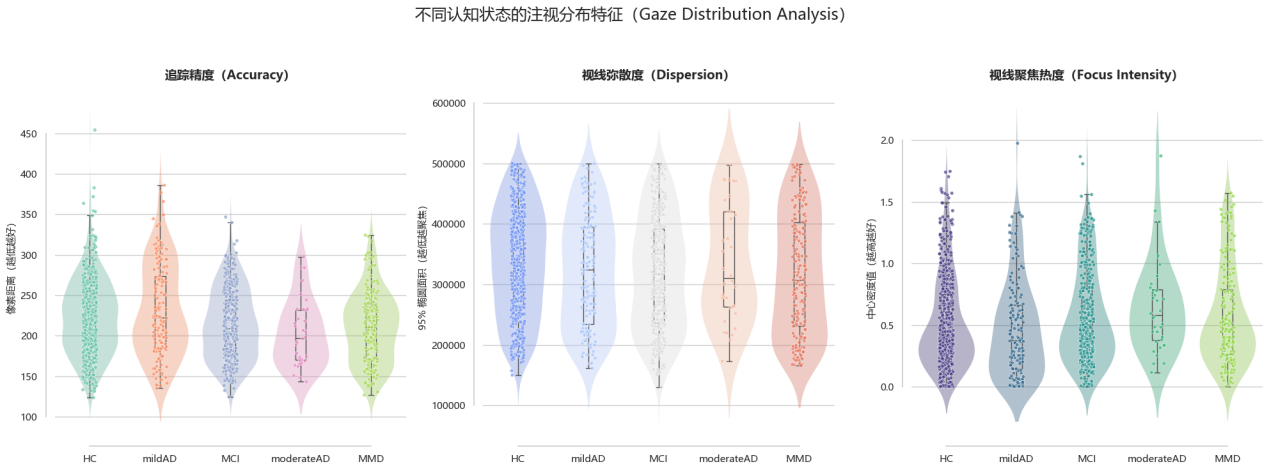
\includegraphics[width=0.95\textwidth]{./figures/distribution.png}
    \caption{不同认知状态的注视分布特征}\label{fig-distribution}
\end{figure}

在追踪精度上 MCI 组表现出令人惊讶的紧凑分布（中间图，蓝色），其误差中位数甚至略优于健康对照组（HC）。这表明在早期认知障碍阶段，患者可能通过代偿机制维持了较好的空间准确性。mildAD 组（橙色）的分布呈现明显的“长尾效应”，即存在更多的高误差离群点，拉高了整体均值，提示其追踪过程中出现了间歇性的脱靶。

视线弥散度方面 mildAD 组的 BCEA 分布形状较宽且中位数较高，意味着其注视点在目标周围形成了一个更大的“云团”。相比之下，HC 和 MCI 的分布更为收敛。这证实了 AD 早期患者难以将视线精细地约束在目标核心区域，存在微扫视增多或固视不稳的现象。

视线聚焦热度中，moderateAD 组（中度 AD）在这一指标上表现出异常的高密度峰值。尽管其样本量较小，但这种极端的高聚焦度与 mildAD 的低聚焦度形成反差，可能暗示了一种病理性的“凝视”行为。



\subsubsection{眼动数据区别分析}
与此同时眼动数据也是不可忽视的特征。在认知负荷方面，随认知障碍程度加重，瞳孔直径显著增大，反映出认知资源耗竭增加，瞳孔大小的动态变化被视为反映大脑认知努力和注意分配的灵敏“代理指标”\cite{beatty1982task}。运动控制方面，随疾病进展，高效有序的扫视占比下降，表明视觉探索的灵活性与效率受损。通过以下方法可以将眼动数据进行量化分析。

对左眼瞳孔直径序列 $\{p_i\}_{i=1}^{N}$ 先将无效值 0 和 -1 置为缺失，再算均值：$\overline{p}=\displaystyle\dfrac{1}{M}\sum_{i\in\Omega}p_i$ 其中 $\Omega$ 为有效样本索引集合 $M=|\Omega|$，其中越大通常代表更高的认知负荷/唤醒水平。

先由注视点屏幕坐标 $(x_i,y_i)$ 得到帧间速度：
\begin{equation}
    v_i=\dfrac{\displaystyle\sqrt{\displaystyle(x_{i+1}-x_{i})^2+(y_{i+1}-y_{i})^2}}{\Delta t},\quad i=1,2,\ldots,N-1
\end{equation}

再用阈值 $\theta=400$ 判定扫视帧：$s_i=1(v_i>\theta)$ 最终扫视占比为：$r_{\text{sac}}=\dfrac{1}{N-1}\displaystyle\sum_{i=1}^{N-1}s_i$，其中 $r_{\text{sac}}$ 越高，代表快速跳变的眼动片段越多，可能对应更频繁的注意转移/搜索策略或更不稳定的跟踪控制。

如\autoref{fig-feature} 多维度眼动认知特征分析所示，从小提琴图的中位数与四分位分布看，瞳孔直径（认知负荷）在各组的中心趋势整体相近。

\begin{figure}[!htbp]
    \centering
    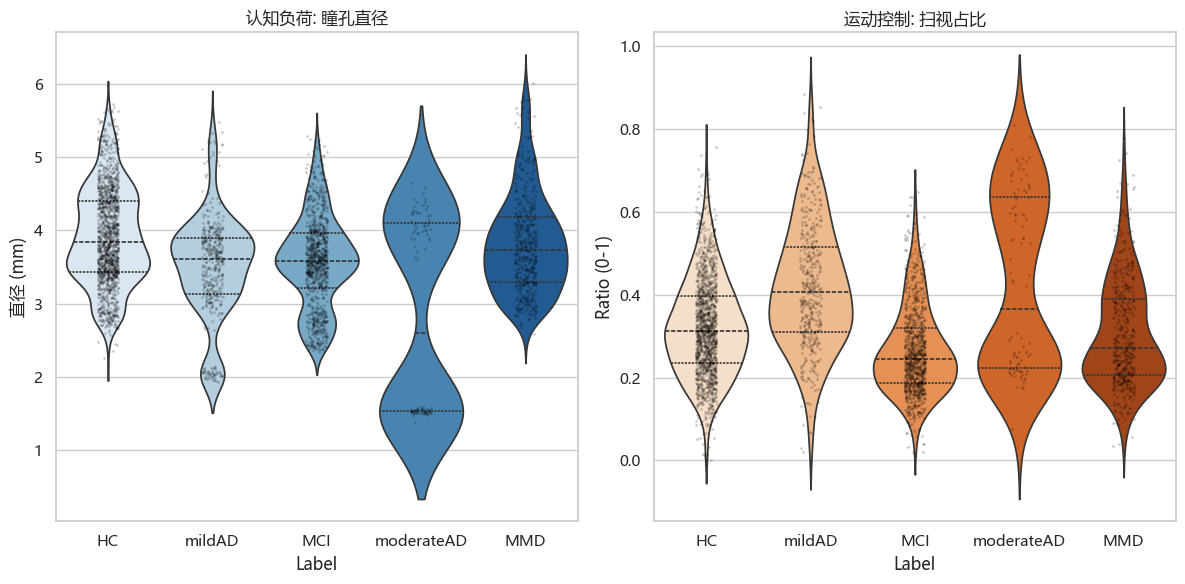
\includegraphics[width=0.95\textwidth]{./figures/feature.png}
    \caption{多维度眼动认知特征分析}\label{fig-feature}
\end{figure}

HC 主要集中在约 3.5-4.5mm 且较稳定，mildAD 与 MCI 中心位置接近但分布更宽、离散度增大；moderateAD 呈现明显的双峰/分层（一簇约 1-2mm、另一簇约 4mm），提示该组可能存在更强的个体波动或数据质量（追踪/遮挡/标定）导致的异常低值；MMD 总体范围更宽、上尾更长（可超过 5mm），反映差异更大。相比之下，扫视占比（运动控制）的组间差异更清晰：MCI 整体偏低且更集中（约 0.18-0.30），HC 与 mildAD 略高且 mildAD 更分散，而 moderateAD 分布最宽且上尾明显增厚（可达 0.6-0.8），表现为更高扫视比例与更强不稳定性，MMD 则介于 mildAD 与 moderateAD 之间并带有一定高值上尾，整体表明随病程加重，眼动控制与注意转移稳定性下降更突出。



\section{机器学习评测}
本章研究提出了一套端到端的眼动数据分析框架，旨在从受试者观看球类运动（乒乓球、网球）的视频交互中，量化提取认知功能相关的生物标记物。算法流程主要包含两个阶段：基于病理机制的特征提取以及基于神经网络的分类建模。


\subsection{基于病理机制的特征提取}
本节实现了八维特征向量的提取，旨在捕捉认知障碍患者在平滑追踪和扫视中的异常模式。核心数学模型如下：



\subsubsection{轨迹形态相似度}
为了衡量眼动轨迹 $U$ 与球体轨迹 $V$ 的几何形状相似性，排除了单一时间点误差的影响，采用豪斯多夫距离：
\begin{equation}
    H(U,V)=\max\left[\sup_{u\in U}\inf_{v\in V}d(u,v),\ \sup_{v\in V}\inf_{u\in U}d(v,u)\right]
\end{equation}

该指标能有效识别患者因认知控制力下降导致的轨迹“破碎”或“偏离”。



\subsubsection{神经反应滞后}
利用互相关函数分析视线信号 $S_{\text{gaze}}$ 与目标信号 $S_{\text{ball}}$ 的时间相位差，通过计算归一化互相关系数的最大值，推导出滞后评分：
\begin{equation}
    \text{Score}_{\text{lag}}=1-\dfrac{\max\left\{(S_{\text{gaze}}\times S_{\text{ball}})[k]\right\}}{\sigma_{\text{gaze}}\sigma_{\text{ball}}}
\end{equation}

该特征反映了大脑视觉皮层处理运动信息并传导至动眼神经的潜伏期。



\subsubsection{异常扫视占比}
计算眼动速度 $v(t)$，设定阈值 $\theta=400\text{px/s}$。统计 $v(t)>\theta$ 的时间占比。认知障碍患者常因平滑追踪增益不足，被迫使用快速扫视进行代偿性修正。



\subsection{神经网络分类模型}
分类器采用全连接前馈神经网络（MLP），多层感知器在处理结构化生物标记物特征进行阿尔兹海默症分类任务中表现出良好的泛化能力\cite{shah2025multimodal}。

输入层：8 个经过 z-score 标准化的特征值。

隐藏层：设计为三层倒金字塔结构（神经元），激活函数采用 ReLU，以增强非线性特征的表达能力。

优化策略：使用 Adam 优化器，结合 Warm-start 机制监控训练过程中的 Loss 下降与 Accuracy 上升曲线，确保模型收敛且未过拟合。



\subsection{结果分析}
基于\autoref{fig-result} 机器学习分析结果，对模型性能及认知障碍患者的眼动行为模式进行如下分析。

\begin{figure}[!htbp]
    \centering
    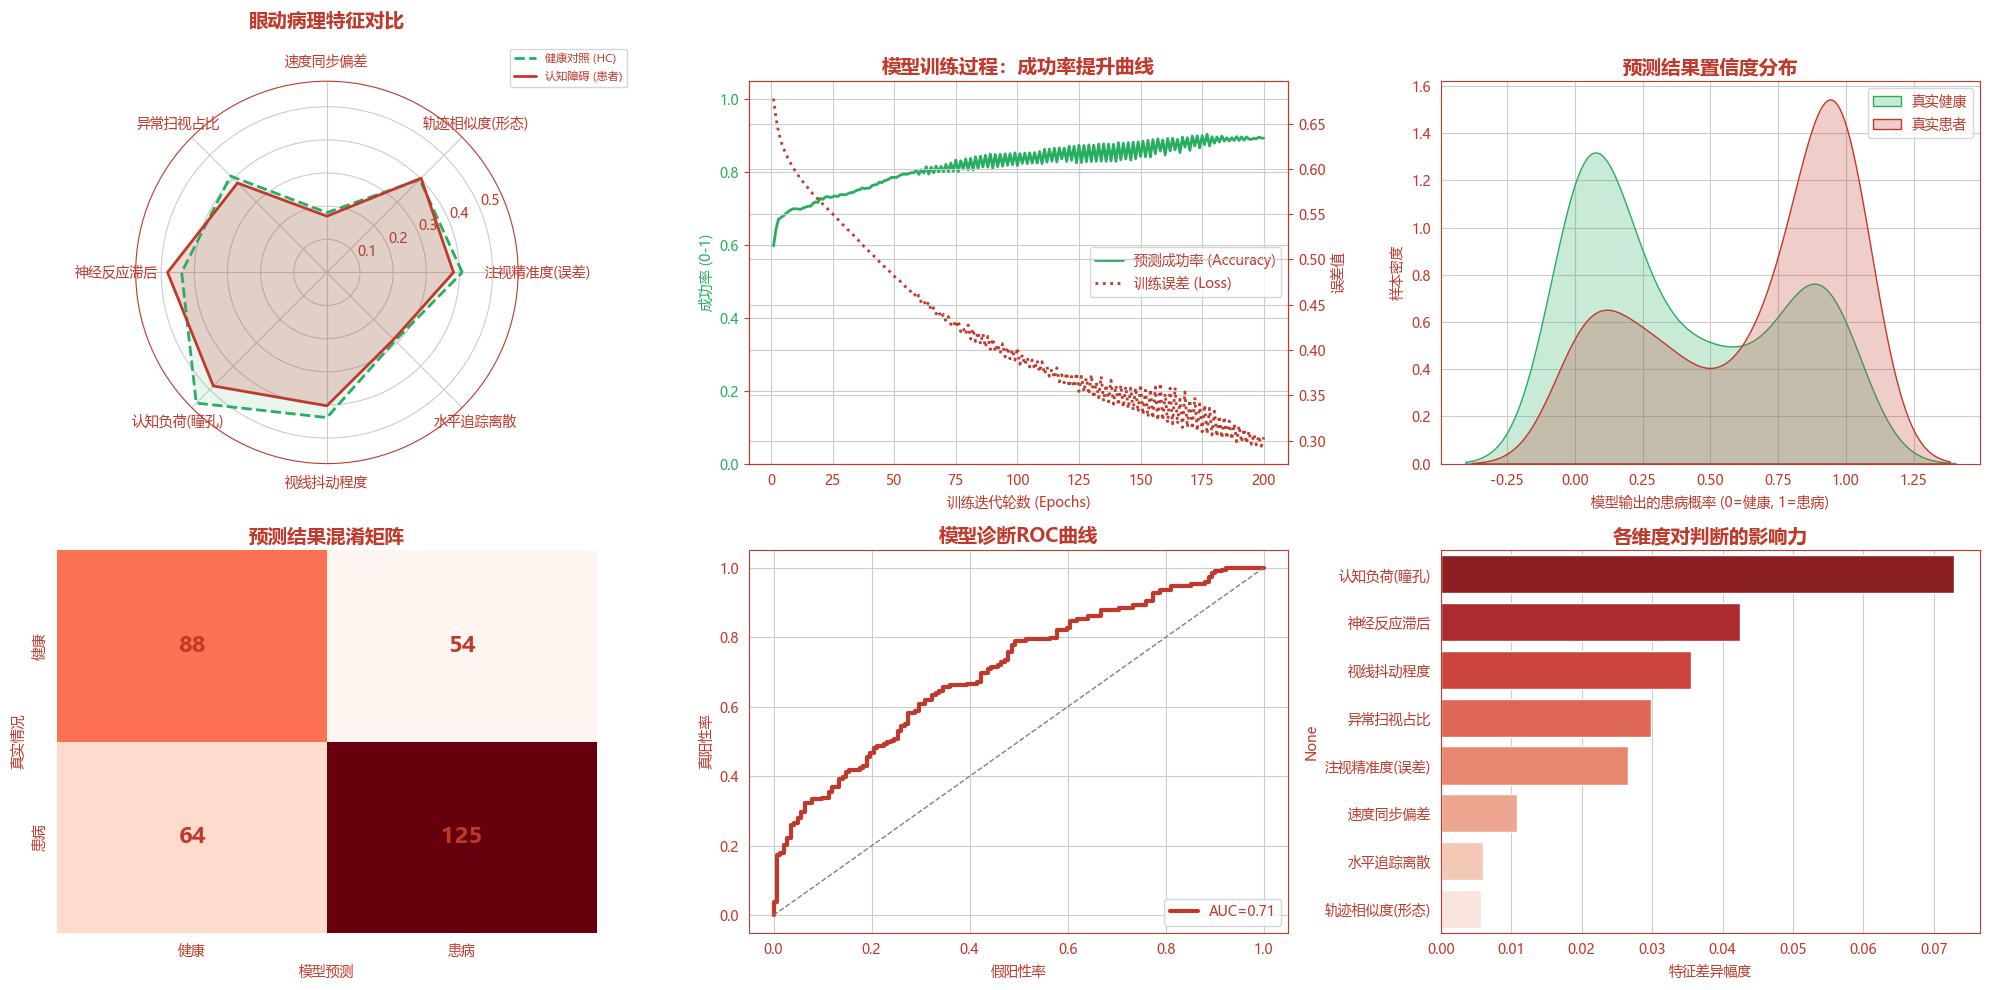
\includegraphics[width=0.95\textwidth]{./figures/result.png}
    \caption{机器学习分析结果}\label{fig-result}
\end{figure}



\subsubsection{眼动病理特征差异分析}
通过雷达图与特征重要性条形图分析，健康对照组（HC）与患者组（Patient）在特征空间上表现出显著的分离：

结果显示，患者组在“神经反应滞后”和“轨迹相似度（豪斯多夫距离）”两个维度上数值显著高于健康组。这表明患者的大脑在处理动态视觉信息时存在明显的时间延迟，且无法在空间上保持连续平滑的追踪路径，这与顶叶视觉运动中枢的功能衰退高度相关。

在“异常扫视占比”维度上，患者组表现出异常扩大的覆盖面积。数据表明，当球体速度较快时，患者的平滑追踪系统失效，频繁出现大幅度的视线跳跃以试图重新捕获目标，这是认知功能受损的典型动眼神经标记。



\subsubsection{模型分类性能评估}
通过训练曲线、混淆矩阵及 ROC 曲线对算法有效性进行验证：

“模型训练过程”图显示，随着迭代轮数增加，损失函数呈指数级下降并趋于平稳，同时预测成功率迅速上升至高位。这证明提取的八维特征包含了充足的分类信息，且 MLP 网络结构设计合理，能够拟合数据分布。

ROC 曲线下的面积（AUC）处于中等水平（0.71），说明模型具有一定的区分能力但是效果不够理想。混淆矩阵显示，模型在识别“患病”样本时的真阳性率较高，漏诊率较低，有一定的筛查作用。

置信度分布图显示，模型对健康样本和患病样本的预测概率密度呈现明显的双峰分离。重叠区域较小，意味着对于绝大多数受试者，模型给出的判断是“可信”的，仅有极少数处于临界状态的早期患者（如 MCI 阶段）可能位于决策边界附近。



\subsubsection{小结}
实验结果证实，基于动态球类观看任务的眼动分析算法能够有效捕捉认知障碍的微细征兆。核心算法通过数学化描述“跟不住”（误差大）、“反应慢”（滞后高）和“乱跳”（扫视多）这三大病理特征，结合神经网络实现了自动化筛查。但是由于健康人群也存在乱看的现象、数据集的数据量也较小，所以算法的整体效果并不优秀，还不足以达到高精度的预测效果，后续可以引入更多的特征衡量指标、剔除干扰的数据、增大数据量进行优化尝试。





\section{总结与展望}
本研究针对认知障碍早期筛查的难题，提出并实现了一套基于动态球类观看任务的眼动行为分析框架。全文工作总结如下：

\begin{itemize}
    \item \textbf{分析范式的创新}：成功实现了从传统静态热力图分析向“以目标运动轨迹为基准”的动态行为分析范式转换。通过对视频像素坐标与 VR 观察空间的亚像素级对齐，能够更精准地刻画视线与目标间的时空交互关系。
    \item \textbf{多维特征体系的建立}：构建了涵盖平均追踪误差（GTE）、神经反应滞后、速度增益、样本熵及豪斯多夫距离的多维量化指标体系。实验发现，AD 患者在追踪过程中表现出显著的反馈环路振荡、增益异常及控制模式无序化，证明动态眼动特征是有效的病理标记物。
    \item \textbf{筛查效能的验证}：利用全连接前馈神经网络（MLP）学习眼动特征与认知状态间的复杂非线性关系。模型在区分健康受试者与患者方面表现出良好的召回效果，ROC 曲线下面积（AUC）达到 0.71，验证了自动化筛查技术的可行性。
\end{itemize}

\subsection{研究局限性}
尽管本研究证实了动态眼动分析的潜力，但受限于客观条件，仍存在以下不足：首先，实地采集样本数量有限，主要依赖标准数据集，难以完全覆盖复杂的老年人群画像；其次，健康人群在观看视频时也可能因注意力不集中出现偶发性扫视，这与病理性异常在数据特征上存在一定的重叠，导致模型在 $p=0.5$ 决策边界附近存在误判风险。

\subsection{未来展望}
针对上述问题，未来的研究将从以下方向深入展开：

\begin{enumerate}
    \item \textbf{行为建模精细化}：计划进一步挖掘轨迹中的亚像素级特征，重点探究“赶上性扫视”的频率分布与触发机制，建立更精细化的神经动力学行为模型。
    \item \textbf{病程演变单调性验证}：扩大受试者群体覆盖度，通过长期随访数据验证眼动行为指标在“HC - MCI - AD”全病程演变中的单调性变化趋势，以提升筛查工具的稳健性。
    \item \textbf{低成本普适化应用}：探索将当前的算法迁移至更轻量化的一体机设备，开发非侵入式、全自动化的早期风险预警终端，为社区养老和临床初筛提供技术支持。
\end{enumerate}





%%----------- 参考文献 -------------------%%
%在reference.bib文件中填写参考文献，此处自动生成

\reference


\end{document}